
\begin{correction} \;
\begin{enumerate}
\item \textbf{\'Etudier les variations de la fonction $f: x\mapsto \ddp\frac{1}{3}x^2-x+3$ associ\'ee:}
\begin{itemize}
\item[$\bullet$] La fonction $f$ est bien d\'efinie sur $\R$ comme fonction polynomiale.
\item[$\bullet$] La fonction $f$ est d\'erivable sur $\R$ comme fonction polynomiale et pour tout $x\in\R$: 
$f^{\prime}(x)=\ddp\frac{2}{3}x-1$.
\item[$\bullet$] On obtient ainsi les variations suivantes:
\begin{center}
\begin{tikzpicture}
 \tkzTabInit{ $x$          /1,%
       $f'(x)$      /1,%
       $f$       /2}%
     { $-\infty$, $\ddp\frac{3}{2}$ ,$+\infty$ }%
  \tkzTabLine {,-,0,+,}%
  \tkzTabVar{
       +/ $+\infty$        /,
        -/$\ddp\frac{9}{4}$           /,%
       +/$+\infty$           /,
                      }
 \tkzTabVal[draw]{2}{3}{0.3}{$3$}{$3$}
 \tkzTabVal[draw]{1}{2}{0.6}{$0$}{$3$}
\end{tikzpicture}
\end{center}
\item[$\bullet$] Les limites en $\pm\infty$ s'obtiennent avec le th\'eor\`{e}me du mon\^{o}me de plus haut degr\'e.
\end{itemize}
\item \textbf{\'Etudier le signe de la fonction $g: x\mapsto f(x)-x=\ddp\frac{1}{3}x^2-2x+3$:}\\
\noindent Le discriminant vaut $\Delta=0$ et l'unique racine est 3. Ainsi

 \fbox{la fonction $g$ est positive sur $\R$ et ne s'annule qu'en 3.}
\item \textbf{Calculer les limites \'eventuelles de la suite $\suiteu$:}\\
\noindent On suppose que la suite $\suiteu$ converge vers un r\'eel $l\in\mathcal{D}_f=\R$.
\begin{itemize}
\item[$\star$] On a donc:
\begin{itemize}
\item[$\circ$] La suite converge vers $l$.
\item[$\circ$] La fonction $f$ est continue sur $\R$ comme fonction polynomiale donc elle est en particulier continue en $l$.
\end{itemize}
Donc d'apr\`{e}s le th\'eor\`{e}me sur les suite et fonction, on obtient que: $\lim\limits_{n\to +\infty} f(u_n)=f(l)$.
\item[$\star$] De plus on a: $\lim\limits_{n\to +\infty} u_{n+1}=l$.
\item[$\star$] On peut donc passer \`{a} la limite dans l'\'egalit\'e: $u_{n+1}=f(u_n)$ et on obtient que: $l=f(l)$/
\item[$\star$] On a donc: $l=f(l)\Leftrightarrow g(l)=0\Leftrightarrow l=3$. \\
\noindent \fbox{La seule limite \'eventuelle est 3.}
\end{itemize}
\item \textbf{Que peut-on dire de la suite $\suiteu$ lorsque $u_0=3$ ou $u_0=0$ ?:}
\begin{itemize}
\item[$\bullet$] Cas 1: si $u_0=3$:\\
\noindent Comme 3 est le point fixe de $f$, on a: $u_1=f(u_0)=f(3)=3$ puis $u_2=f(u_1)=f(3)=3$... On montre alors par r\'ecurrence que

 \fbox{la suite $\suiteu$ est constante \'egale \`{a} 3 et donc qu'elle converge vers 3.}
\item[$\bullet$] Cas 2: si $u_0=0$:\\
\noindent On a par d\'efinition de la suite: $u_1=f(u_0)=f(0)=3$. Mais comme 3 est le point fixe de la fonction $f$, on a alors $u_2=f(u_1)=f(3)=3$ puis $u_3=f(u_2)=f(3)=3$... On montre alors par r\'ecurrence sur $n\geq 1$ que 

\fbox{la suite $\suiteu$ est stationnaire \'egale \`{a} 3 et donc qu'elle converge vers 3.} 
\end{itemize}
\item \textbf{On suppose que $u_0\in\rbrack 0,3\lbrack$.}
\begin{enumerate}
\item \textbf{Montrer que la suite est bien d\'efinie et que pour tout $n\in\N$: $u_n\in\rbrack 0,3\lbrack$:}\\
\noindent 
On peut commencer par montrer que l'intervalle $\rbrack 0,3\lbrack$ est stable par $f$. On traite ici les intervalles $\left\rbrack 0,\ddp\frac{3}{2}\right\rbrack$ et  $\left\lbrack \ddp\frac{3}{2},3\right\lbrack$ s\'eparemment.\\
La fonction $f$ est strictement d\'ecroissante sur $\left\rbrack 0,\ddp\frac{3}{2}\right\rbrack$, et $f( 0)=3$, $f\left( \ddp\frac{3}{2}\right)=\ddp\frac{9}{4}$. Donc pour tout $x \in \left\rbrack 0,\ddp\frac{3}{2}\right\rbrack, f(x) \in \left\rbrack \ddp \frac{9}{4},\ddp\frac{3}{2}\right\rbrack$, donc $f(x) \in \rbrack 0,3\lbrack$.\\
La fonction $f$ est strictement croissante sur $\left\lbrack \ddp\frac{3}{2},3\right\lbrack$, et $f\left(3\right)=3$, $f\left( \ddp\frac{3}{2}\right)=\ddp\frac{9}{4}$. Donc pour tout $x \in \left\lbrack \ddp\frac{3}{2},3\right\lbrack, f(x) \in \left\rbrack \ddp \frac{9}{4},3\right\rbrack$, donc $f(x) \in \rbrack 0,3\lbrack$.\\
Ainsi, pour tout $x \in \rbrack 0,3\lbrack, f(x) \in \rbrack 0,3\lbrack$, et donc l'intervalle $\rbrack 0,3\lbrack$ est stable par $f$.\\
%\begin{itemize}
%\item[$\circ$] La fonction $f$ est continue sur $\left\rbrack 0,\ddp\frac{3}{2}\right\rbrack$.
%\item[$\circ$] La fonction $f$ est strictement d\'ecroissante sur $\left\rbrack 0,\ddp\frac{3}{2}\right\rbrack$.
%\item[$\circ$] $f( 0)=3$ et $f\left( \ddp\frac{3}{2}\right)=\ddp\frac{9}{4}$.
%\end{itemize}
%Ainsi d'apr\`{e}s le th\'eor\`{e}me de la bijection, on a en particulier que $f(\left\rbrack 0,\ddp\frac{3}{2}\right\rbrack)=\left\lbrack \ddp\frac{9}{4},3\right\lbrack$. \\
%\noindent On a aussi:
%\begin{itemize}
%\item[$\circ$] La fonction $f$ est continue sur $\left\lbrack \ddp\frac{3}{2},3\right\lbrack$.
%\item[$\circ$] La fonction $f$ est strictement croissante sur $\left\lbrack \ddp\frac{3}{2},3\right\lbrack$.
%\item[$\circ$] $f\left(3\right)=3$ et $f\left( \ddp\frac{3}{2}\right)=\ddp\frac{9}{4}$.
%\end{itemize}
%Ainsi d'apr\`{e}s le th\'eor\`{e}me de la bijection, on a en particulier que $f(\left\lbrack \ddp\frac{3}{2},3\right\lbrack)=\left\lbrack \ddp\frac{9}{4},3\right\lbrack$. \\
%\noindent Au final on obtient donc que: 
%$$f(\rbrack 0,3\lbrack)=f(\left\rbrack 0,\ddp\frac{3}{2}\right\rbrack)\cup f(\left\lbrack \ddp\frac{3}{2},3\right\lbrack)=\left\lbrack \ddp\frac{9}{4},3\right\lbrack\cup\left\lbrack \ddp\frac{9}{4},3\right\lbrack=\left\lbrack \ddp\frac{9}{4},3\right\lbrack.$$
%Et comme $\left\lbrack \ddp\frac{9}{4},3\right\lbrack \subset \rbrack 0,3\lbrack$, \fbox{l'intervalle $\rbrack 0,3\lbrack$ est stable par $f$.} 
On montre par r\'ecurrence sur $n\in\N$ la propri\'et\'e : $\mathcal{P}(n):\ u_n\ \hbox{existe et}\ u_n\in\rbrack 0,3\lbrack.$
\begin{itemize}
\item[$\star$] Initialisation: pour $n=0$:\\
\noindent Par d\'efinition de la suite, on a bien que $u_0$ existe et $u_0\in\rbrack 0,3\lbrack$. Donc $\mathcal{P}(0)$ est vraie.
\item[$\star$] H\'er\'edit\'e: soit $n\in\N$ fix\'e, on suppose que la propri\'et\'e vraie \`{a} l'ordre $n$, montrons que $\mathcal{P}(n+1)$ est vraie.
\begin{itemize}
\item[$\circ$] Par hypoth\`{e}se de r\'ecurrence, on sait que $u_n$ existe et que $u_n\in\rbrack 0,3\lbrack$. En particulier $u_n$ existe et $u_n\in\mathcal{D}_f$. Donc $f(u_n)$ existe c'est-\`{a}-dire $u_{n+1}$ existe.
\item[$\circ$] Par hypoth\`{e}se de r\'ecurrence, on sait que $u_n$ existe et que $u_n\in\rbrack 0,3\lbrack$. Or l'intervalle $\rbrack 0,3\lbrack$ est stable par $f$. Donc $f(u_n)\in\rbrack 0,3\lbrack$ c'est-\`{a}-dire $u_{n+1}\in\rbrack 0,3\lbrack$.
\end{itemize}
Donc $\mathcal{P}(n+1)$ est vraie.
\item[$\star$] Conclusion: il r\'esulte du principe de r\'ecurrence que 


\fbox{la suite $\suiteu$ est bien d\'efinie et que pour tout $n\in\N,\ u_n\in\rbrack 0,3\lbrack.$}
\end{itemize}
\item \textbf{\'Etudier la monotonie de la suite $\suiteu$:}\\
\noindent Soit $n\in\N$, on a: $u_{n+1}-u_n=f(u_n)-u_n=g(u_n)$. Ainsi comme le signe de $g$ est positif sur $\R$, on obtient que pour tout $n\in\N$: $u_{n+1}-u_n\geq 0$. Ainsi \fbox{la suite $\suiteu$ est croissante.}
\item \textbf{\'Etudier le comportement \`{a} l'infini de la suite $\suiteu$:}
\begin{itemize}
\item[$\star$] La suite $\suiteu$ est croissante et major\'ee par 3 donc d'apr\`{e}s le th\'eor\`{e}me sur les suites monotones, elle converge.
\item[$\star$] Comme la seule limite \'eventuelle est 3, \fbox{la suite $\suiteu$ converge vers 3.}
\end{itemize}
\end{enumerate}
\item \textbf{On suppose que $u_0>3$.}
\begin{enumerate}
\item \textbf{Montrer que la suite est bien d\'efinie et que pour tout $n\in\N$: $u_n>3$:}\\
\noindent On peut commencer par montrer que l'intervalle $\rbrack 3,+\infty\lbrack$ est stable par $f$. On a $f$ strictement croissante sur $\rbrack 3,+\infty\lbrack$, et $f(3) = 3$, donc pour tout $x \in \rbrack 3,+\infty\lbrack$, $f(x) >3$ et l'intervalle $\rbrack 3,+\infty\lbrack$ est stable par $f$.
%\begin{itemize}
%\item[$\circ$] La fonction $f$ est continue sur $\rbrack 3,+\infty\lbrack$.
%\item[$\circ$] La fonction $f$ est strictement croissante sur $\rbrack 3,+\infty\lbrack$.
%\item[$\circ$] $f(3)=3$ et $\lim\limits_{x\to +\infty} f(x)=+\infty$.
%\end{itemize}
%Ainsi d'apr\`{e}s le th\'eor\`{e}me de la bijection, on a en particulier que $f(\rbrack 3,+\infty\lbrack)=\rbrack 3,+\infty\lbrack$. Et comme $\rbrack 3,+\infty\lbrack \subset \rbrack 3,+\infty\lbrack$, \fbox{l'intervalle $\rbrack 3,+\infty\lbrack$ est stable par $f$.} 
\begin{itemize}
\item[$\star$] On montre par r\'ecurrence sur $n\in\N$ la propri\'et\'e
$$\mathcal{P}(n):\ u_n\ \hbox{existe et}\ u_n>3.$$
\item[$\star$] Initialisation: pour $n=0$:\\
\noindent Par d\'efinition de la suite, on a bien que $u_0$ existe et $u_0>3$. Donc $\mathcal{P}(0)$ est vraie.
\item[$\star$] H\'er\'edit\'e: soit $n\in\N$ fix\'e, on suppose que la propri\'et\'e vraie \`{a} l'ordre $n$, montrons que $\mathcal{P}(n+1)$ est vraie.
\begin{itemize}
\item[$\circ$] Par hypoth\`{e}se de r\'ecurrence, on sait que $u_n$ existe et que $u_n>3$. En particulier $u_n$ existe et $u_n\in\mathcal{D}_f$. Donc $f(u_n)$ existe c'est-\`{a}-dire $u_{n+1}$ existe.
\item[$\circ$] Par hypoth\`{e}se de r\'ecurrence, on sait que $u_n$ existe et que $u_n>3$. Or l'intervalle $\rbrack 3,+\infty\lbrack$ est stable par $f$. Donc $f(u_n)>3$ c'est-\`{a}-dire $u_{n+1}>3$.
\end{itemize}
Donc $\mathcal{P}(n+1)$ est vraie.
\item[$\star$] Conclusion: il r\'esulte du principe de r\'ecurrence que

 \fbox{la suite $\suiteu$ est bien d\'efinie et que pour tout $n\in\N,\ u_n>3.$}
\end{itemize}
\item \textbf{\'Etudier la monotonie de la suite $\suiteu$:}\\
\noindent Soit $n\in\N$, on a: $u_{n+1}-u_n=f(u_n)-u_n=g(u_n)$. Ainsi comme le signe de $g$ est positif sur $\R$, on obtient que pour tout $n\in\N$: $u_{n+1}-u_n\geq 0$. Ainsi \fbox{la suite $\suiteu$ est croissante.}
\item \textbf{\'Etudier le comportement \`{a} l'infini de la suite $\suiteu$:}
\begin{itemize}
\item[$\star$] La suite $\suiteu$ est croissante donc d'apr\`{e}s le th\'eor\`{e}me sur les suites monotones, elle converge ou elle diverge vers $+\infty$.
\item[$\star$] On suppose par l'absurde que la suite $\suiteu$ converge vers un r\'eel $l$. On a alors:
\begin{itemize}
\item[$\circ$] La suite $\suiteu$ converge vers $l$.
\item[$\circ$] Comme la suite $\suiteu$ est croissante, on a pour tout $n\in\N$: $u_n\geq u_0$.
\end{itemize}
D'apr\`{e}s le th\'eor\`{e}me de passage \`{a} la limite, on obtient donc que: $l\geq u_0$. Or par hypoth\`{e}se, on sait que $u_0>3$. Ainsi on obtient que: $l>3$. Absurde car la seule limite \'eventuelle de la suite $\suiteu$ est 3. Ainsi \fbox{la suite $\suiteu$ diverge vers $+\infty$.}
\end{itemize}
\end{enumerate} 
\item \textbf{On suppose que $u_0<0$.}
\begin{enumerate}
\item \textbf{Montrer que $u_1>3$:}\\
\noindent On a:
\begin{itemize}
\item[$\star$] La fonction $f$ est continue sur $\rbrack -\infty,0\lbrack$ comme fonction polynomiale.
\item[$\star$] La fonction $f$ est strictement d\'ecroissante sur $\rbrack -\infty,0\lbrack$.
\item[$\star$] $\lim\limits_{x\to -\infty}f(x)=+\infty$ et $f(0)=3$
\end{itemize}
Ainsi d'apr\`{e}s le th\'eor\`{e}me de la bijection, on a en particulier que $f(\rbrack -\infty,0\lbrack)=\left\rbrack 3,+\infty\right\lbrack$. Or on a suppos\'e que $u_0\in\rbrack -\infty,0\lbrack$ donc $f(u_0)\in \left\rbrack 3,+\infty\right\lbrack$, \`{a} savoir $u_1\in \left\rbrack 3,+\infty\right\lbrack$. Donc on a bien \fbox{$u_1>3.$}
\item \textbf{En d\'eduire le comportement \`{a} l'infini de la suite $\suiteu$:}\\
\noindent La suite $(u_n)_{n\geq 1}$ a donc un terme initial $u_1>3$. Ainsi la suite $(u_n)_{n\geq 1}$ se comporte comme la suite de la question 5 et en particulier elle diverge vers $+\infty$. Mais le comportement \`{a} l'infini d'une suite ne d\'epend pas de ses premiers termes donc \fbox{la suite $\suiteu$ diverge vers $+\infty$.}
\end{enumerate} 
\end{enumerate}
\end{correction}